\section{Parsing}
Processing an input text consists generally in, verifying that the
structure of the text is correct, and in performing some operations
using the text under analysis.\\

In general, a grammar describes the syntactical structure of the
input text. Thus, verifying that the structure of the text is correct
consists in making sure that the text is in conformity with the
grammar. This is \textbf{parsing}.\\

The parsing operation is divided into two activities:
\begin{enumerate}
  \item Lexical analysis
  \item Syntax analysis
\end{enumerate}
\subsection{Lexical Analysis}
The \textbf{lexical analysis} activity consists in reading a text character by
character and in grouping the characters that form terminals of the
grammar. Such terminals are usually called \textbf{tokens}. E.g.
\begin{itemize}
  \item Identifiers of programming languages, such as \texttt{anItem}, \texttt{n}
  \item Keywords of programming languages, such as \texttt{if}, \texttt{extends}
  \item Various numerical constants
  \item Character strings such as \texttt{"This is a comment"}, \texttt{"Yes"}
  \item Specific tokens such as \texttt{(}, \texttt{=}, etc.
\end{itemize}
Between terminals lie separators, such as blank spaces, tabs, new lines, and comments,
which are all usually ignored.
We usually use \texttt{lexers} or \texttt{scanners}, which are programs that perform 
the lexical analysis of an input text. The implementation of lexers 
is generally based on the use of regular expressions and/or FSAs. Some lexer tools
include \texttt{lex}, \texttt{flex}, \texttt{jflex}, anf more.
\subsection{Syntax Analysis}
The second activity of parsing consists in verifying that the input text is well constructed, i.e.
the input is in conformity with a given
grammar.
For the verification of the conformity with respect of a given
grammar, we build the parse tree of the input text.\\

An input text is syntactically correct iff the parse tree can be built.\\

A program that performs this activity is called a \textbf{parser}. The main
task of a parser is to create the parse tree of its input using a
grammar that describes the structure of its input. Note that a
parser uses a lexer for the lexical analysis.\\

Parse trees graphically illustrate how a given word is generated by a grammar, i.e. 
which productions are used to generate a given word.

\subsubsection{Bottom-Up Analysis}
One approach to generate a parse tree of an input according to a given grammar is the \textbf{bottom-up analysis}.
\begin{figure}[H]
  \centering
  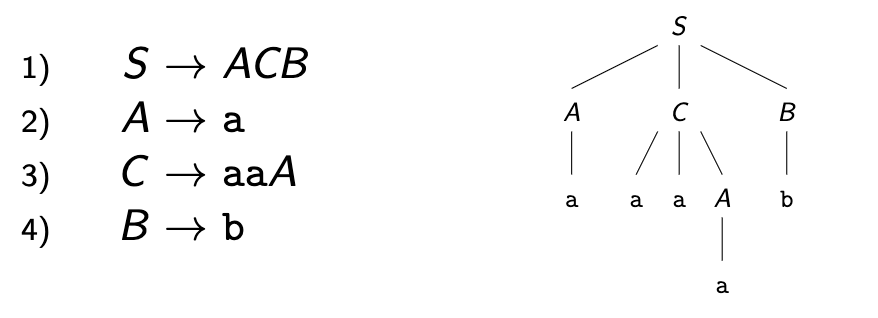
\includegraphics[width=\columnwidth]{parsing-1}
\end{figure}
The parse tree of the input $aaaab$ can be constructed from the terminals
using the rules 2) twice and 4) once, then rule 3) and finally rule 1).
\subsubsection{Top-Down Analysis}
The second approach called \textbf{top-down analysis} consists in applying derivations successively from the first
rewriting rule or axiom. This approach is easier but has some limitations.
\begin{figure}[H]
  \centering
  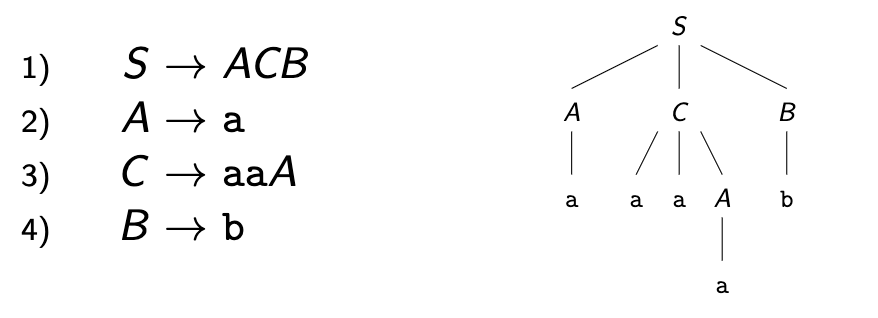
\includegraphics[width=\columnwidth]{parsing-1}
\end{figure}
\subsubsection{Recursive Descent}
\textbf{Recursive Descent} is a top-down approach in which we execute a programm that applies a set 
of recursive functions to process the input. This may involve backtracking, but we will try
to get rid of it, for efficiency and simplification reasons.
\begin{figure}[H]
  \centering
  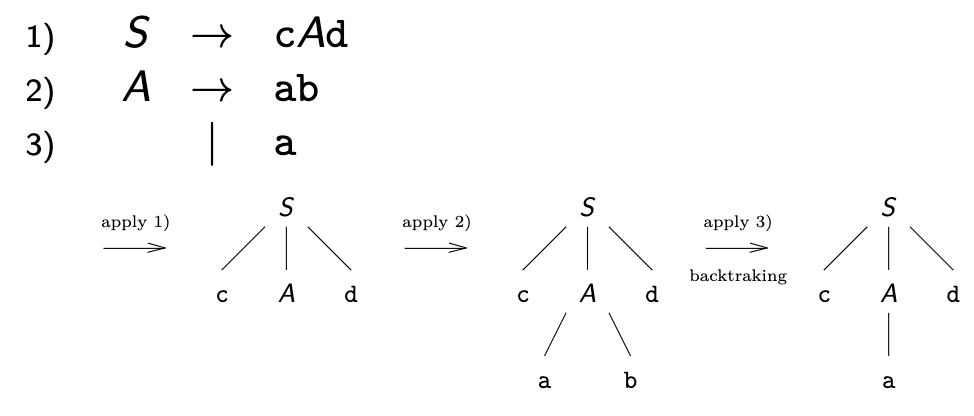
\includegraphics[width=\columnwidth]{parsing-2}
\end{figure}
\subsection{Classes of Context-free Grammars}
The class of LL(1) grammars is a subset of context-free
grammars. One way of parsing such grammars is to use recursive
descent parsers in which no backtracking is required.
\begin{itemize}
\item LL(1) stands for Left to right Left-most derivation with 1
token lookahead.
\item LL(1) is one of the easiest (sometimes fastest) techniques.
\item A recursive descent parser has a parsing function (or method)
for each non terminal that can recognize any sequences of
tokens generated by that nonterminals.
\item The idea of a recursive descent parser it to use the current
input token to decide which alternative to choose.
\end{itemize}
Left-most derivation means that the left-most rule is used (expanded) first.
For example the word $acbb$ gets recognized as follows:
\begin{figure}[H]
  \centering
  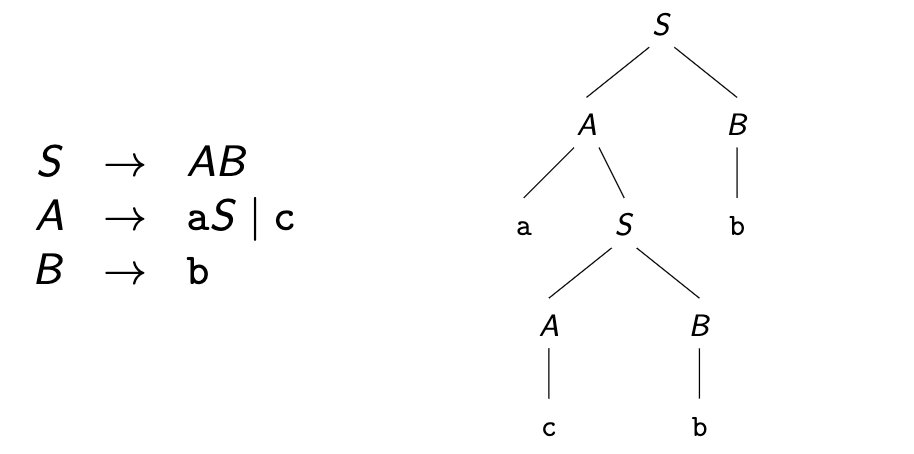
\includegraphics[width=\columnwidth]{parsing-3}
\end{figure}
Left-most derivation visits the nodes of a parse tree according to the DFS algorithm.
The main problem of recursive descent is \textbf{left-recursion}, which causes 
the parser to enter into an infinite recursion.\\

\subsubsection{Left-recursion}
Left recursion has \textbf{immediate left-recursion} if it has the form
\begin{align*}
  X \rightarrow X\alpha \mid \beta
\end{align*} 
or more generally
\begin{align*}
  X \rightarrow & X\alpha_1  \mid \dots X\alpha_n \mid \beta_1
   \mid \dots \mid \beta_n
\end{align*} 
\textbf{General left-recursion} can occur through several rules for example:
\begin{align*}
  S & \rightarrow Aa \mid b\\
  A & \rightarrow Ac \mid Sd \mid \epsilon
\end{align*}
To remove immediate left-recursion, auxiliary rules are required, e.g.:
\begin{align*}
  X \rightarrow & X\alpha_1  \mid \dots X\alpha_n \mid \beta_1
   \mid \dots \mid \beta_n
\end{align*} 
becomes 
\begin{align*}
  X \rightarrow & \beta_1 X' \mid \dots \mid \beta_n X'\\
  X' \rightarrow & \alpha_1X' \mid \dots \mid \alpha_n X' \mid \epsilon
\end{align*}

\subsubsection{Left-factoring}
When two or more grammar rule choices share a common prefix,
LL(1) parsers cannot determine which choice to use or which part
has to be expanded:
\begin{align*}
  X \rightarrow \alpha \beta \mid \alpha \gamma
\end{align*}
To solve this, we can factorize the common prefix:
\begin{align*}
  X \rightarrow \alpha X'\\
  X' \rightarrow \beta \mid \gamma
\end{align*}
\subsection{LL Grammars}
A grammar is LL(1) iff there exists a recursive descent parser with
1 token lookahead for this grammar (top-down analysis).
A grammar is LL($k$) iff there exists a recursive descent parser that
uses $k$ tokens lookahead.\\

The class of LL($k$) grammars strictly includes the class LL($k - 1$),
  where ($k > 1$); in other words there are LL($k$) grammars for which
  no LL($k - 1$) grammar exists. In other words LL($k$) parser are
  more powerful than LL($k - 1$) parsers.\\

  Fortunately most LL(k) grammars can be translated into
  LL(1) grammar, but not all.

\subsection{LR Grammars}
LR(1), LR($k$) grammars can be analyzed with parsers based on the
bottom-up technique with 1 token lookahead, $k$ token lookahead
respectively.
LR($k$) stands for Left to right Right-most derivation with k tokens
lookahead.
Bottom-up parsers are much more powerful than top-down parsers.
It has been shown that any LR($k$) grammar ($k > 0$) can be
translated into a LR(1) grammar.\\

\subsection{Comparison of LL and LR Parsers}
The following shows the relationships between LL and LR:
\begin{figure}[H]
  \centering
  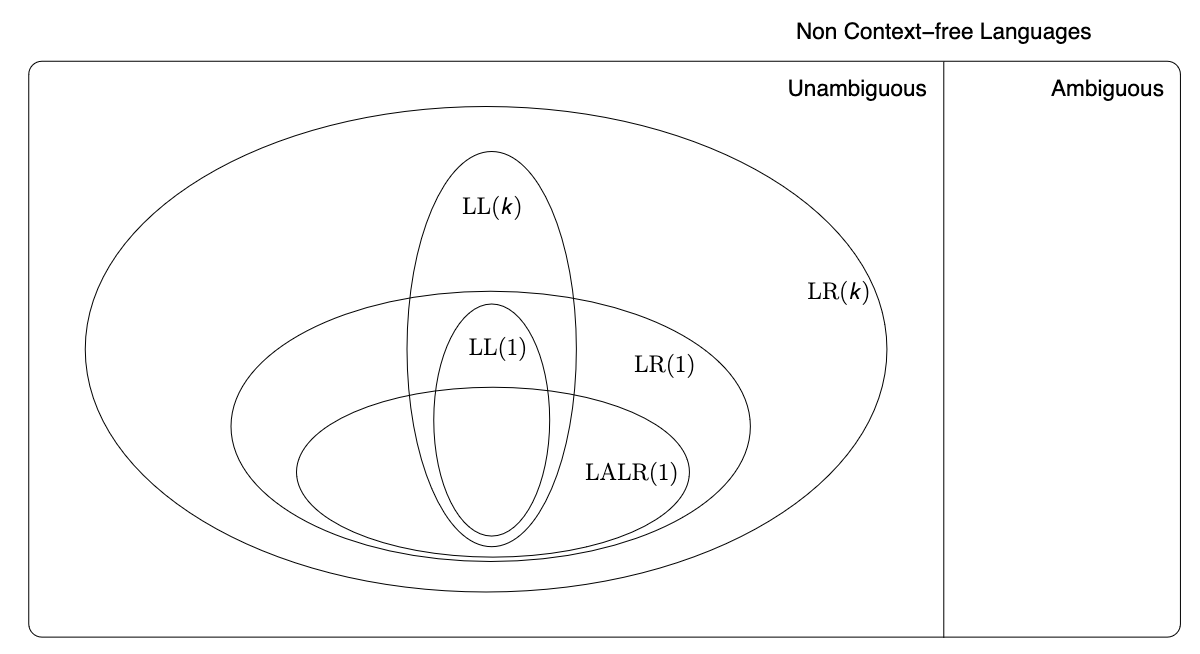
\includegraphics[width=\columnwidth]{parsing-4}
\end{figure}

LR parsers are (disadvantages of LR vs LL):
\begin{itemize}
  \item Much more complex than LL parsers
  \item More difficult to use
  \item Less efficient
  \item Require much more space than LL parsers
  \item Only used through parser generators. Due to 
        the size of tables of LR parsers, parser generators only work for a sub-class of LR grammars called LALR
        (lookahead LR)
\end{itemize}
LR parsers are (advantages of LR vs LL):
\begin{itemize}
  \item Left-recursion is allowed (grammars are easier to read)
  \item More complex context-free languages can be analyzed
  \item Errors are detected as soon as they are encountered
  \item Almost all programming languages can be parsed by bottom-up parsers
\end{itemize}